\documentclass{article}

% Language setting
% Replace `english' with e.g. `spanish' to change the document language
\usepackage[greek,english]{babel} 
\usepackage{alphabeta}
%\usepackage[english]{babel}

% Set page size and margins
% Replace `letterpaper' with `a4paper' for UK/EU standard size
\usepackage[letterpaper,top=2cm,bottom=2cm,left=3cm,right=3cm,marginparwidth=1.75cm]{geometry}


% Useful packages
% \usepackage{listings}
% \usepackage{subcaption}
\usepackage{tikz}
% \usepackage{multirow}

\usepackage{mathtools}
\usepackage{enumerate}
\usepackage{amsmath}
\usepackage{graphicx}
\usepackage[colorlinks=true, allcolors=blue]{hyperref}

\title{Προσομοίωση και Μοντελοποίηση Δυναμικών Συστημάτων ΑΠΘ Main Project}
\author{Σταύρος Βασίλειος Μπουλιόπουλος 9671 smpoulio@ece.auth.gr}

\begin{document}
\maketitle

% \begin{abstract}
% Your abstract.
% \end{abstract}

\section{Εισαγωγή}

Στο πλαίσιο της τρίτης εργασίας του μαθήματος μας ζητήθηκε να αναγνωρίσουμε το άγνωστο γραμμικό σύστημα (S) με μετρήσιμα σήματα μόνο την είσοδο και την έξοδο του συστήματος γνωρίζοντας ότι το (S) είναι ευσταθές και αιτιατό. Γι'αυτόν τον λόγο, διερεύνησαμε την γραμμικότητα του συστήματος για να προσδιορίσουμε την δομή του μοντέλου,έτσι ώστε να προσομοιώσουμε τις μεθόδους προσδιορισμού των παραμέτρων του μοντέλου στην MATLAB και να εξάγουμε συμπεράσματα βάσει διαγραμμάτων και συντελεστών αξιολόγησης. 

\begin{center}

 \begin{tikzpicture}[scale=1]
\draw (0,0) node[rectangle,inner sep=18pt,draw] (s) {Σύστημα (S)};
\draw[->] (s.east) -- ++(1,0) node[right] {$y(t)$};
\draw[<-] (s.west) -- ++(-1,0) node[left] {$u(t)$};

\draw[->,black] (s) ++(0.2,-2) node[below] {Νόμος $T, H$} to[bend left] (s);
\end{tikzpicture}
\end{center}


% \begin{figure}[!htb]
%   \centering
%   {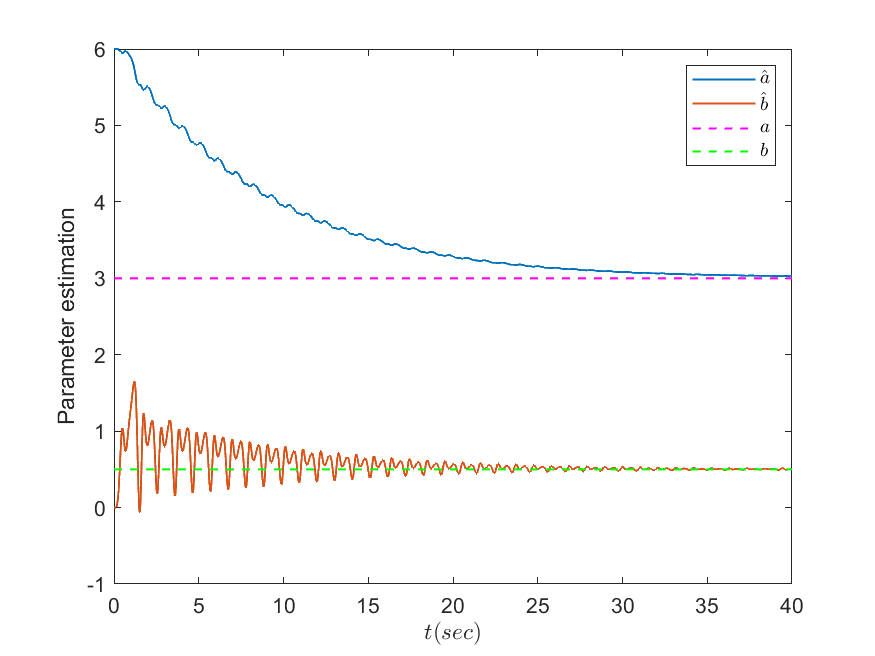
\includegraphics[width=0.4\textwidth]{prob1_b_params_est.png}} 
%   % \subfigure(a){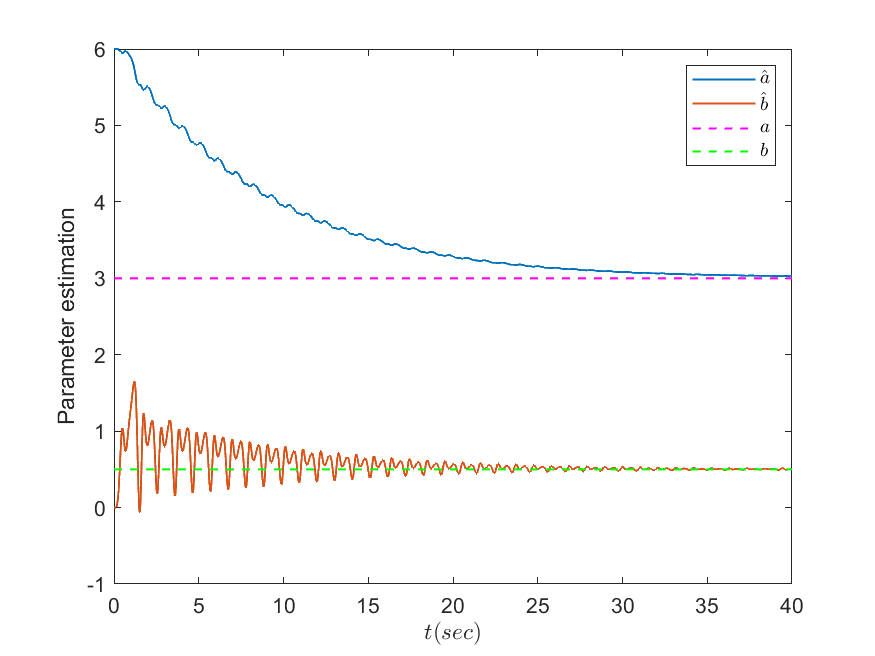
\includegraphics[width=0.4\textwidth]{prob1_b_params_est.png}} 
%   % \subfigure(b){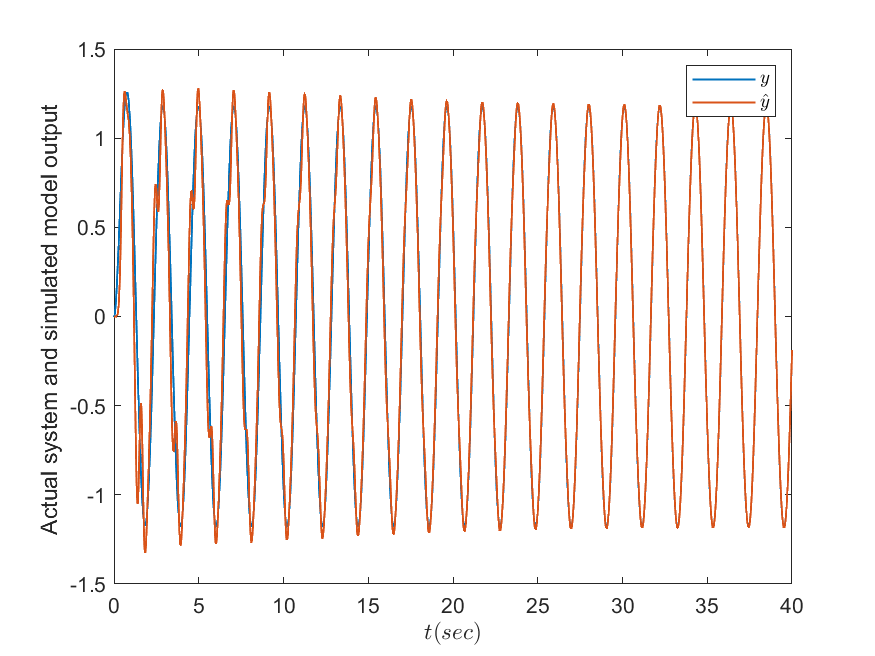
\includegraphics[width=0.4\textwidth]{prob1_b_outputs.png}} 
%   % \subfigure(c){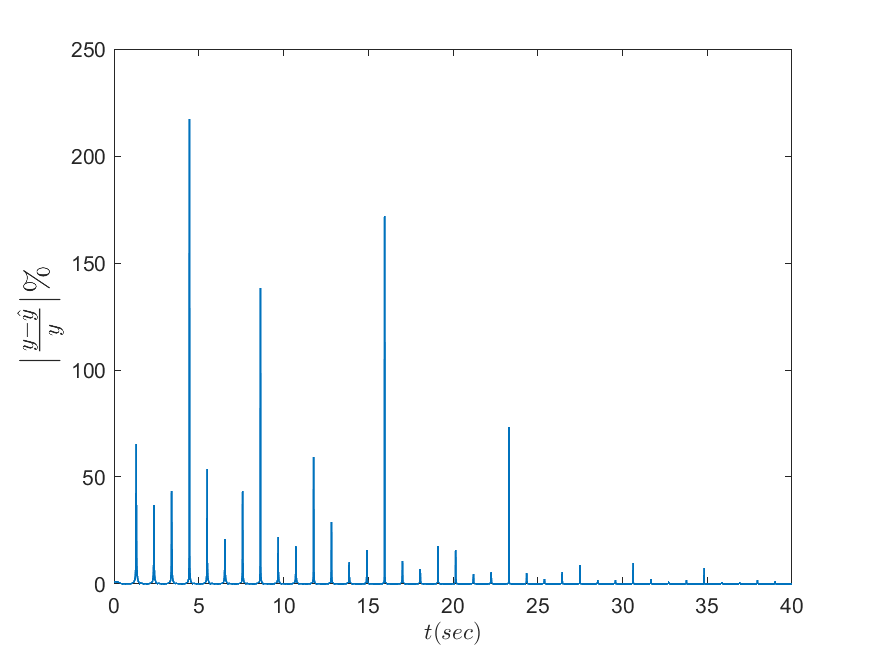
\includegraphics[width=0.4\textwidth]{prob1_b_errorPERC.png}}
%   % \subfigure(d){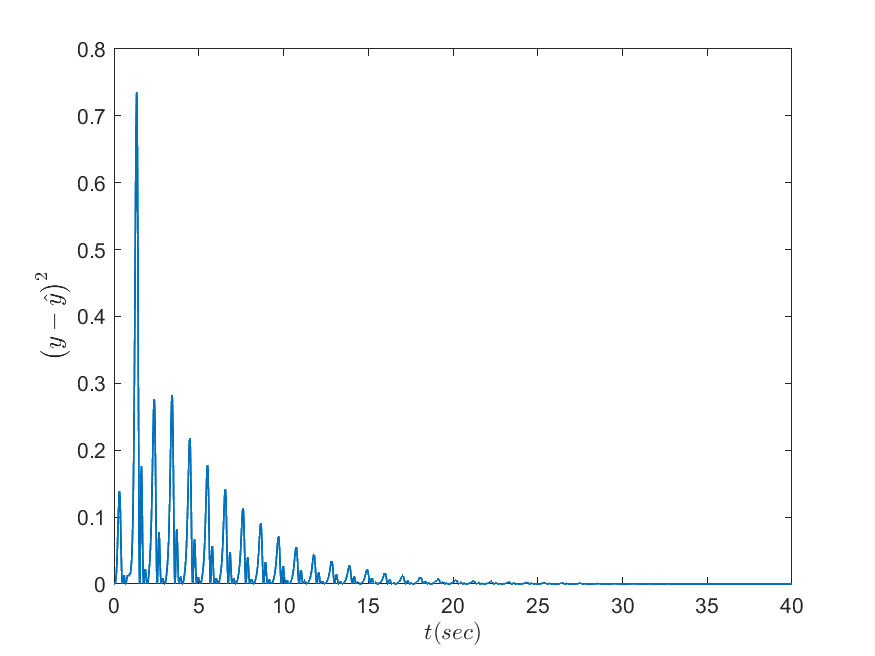
\includegraphics[width=0.4\textwidth]{prob1_b_errorMSE.png}}

%   \caption{(a) Εκτίμηση και σύγκλιση παραμέτρων (b) Έξοδος συστήματος (c) Ποσοστιαίο σφάλμα(d) Μέσο τετραγωνικό σφάλμα}
 
% \label{fig:foobar2}
% \end{figure}

\section{Ερώτημα Α) Ανάλυση γραμμικότητας συστήματος}

Στο πρώτο ερώτημα της εργασίας αποδείξαμε ότι το σύστημα ακολουθεί γραμμική συμπεριφορά σε ικανοποιητικό επίπεδο βάσει των αρχών επαλληλίας και ομοιογένειας: \newline
\begin{itemize}
    \item Νόμος Τ: Έστω οι έξοδοι 
    \begin{equation*}
    y_1(t) = T\left[u_1(t)\right]
    \end{equation*}
    \begin{equation*}
    y_2(t) = T\left[u_2(t)\right]
    \end{equation*}
    το σύστημα επιβεβαιώνει την αρχή επαλληλίας αν και μόνο αν: 
    \begin{equation*}
    T\left[u_1(t) + u_2(t)\right] = T\left[u_1(t)\right] + T\left[u_2(t)\right]
    \end{equation*}

    κατά την προσομοίωση επιλέγουμε τις εισόδους: 
    \begin{equation*}
    \boxed{
    u_1 = cos(t)
    }
    \end{equation*}
    \begin{equation*}
    \boxed{
    u_2 = 2 \cdot cos(2 \cdot t)
    }
    \end{equation*}
    \begin{equation*}
    \boxed{
    u_{12} = u_1 + u_2 = cos(t) + 2 \cdot cos(2 \cdot t)
    }
    \end{equation*}
    παίρνουμε τις εξόδους απο το αρχείο \textit{sys.p}:
    \begin{equation*}
    \boxed{
    y_1(t) = T\left[u_1(t)\right]
    }
    \end{equation*}
    \begin{equation*}
    \boxed{
    y_1(t) = T\left[u_2(t)\right]
    }
    \end{equation*}
    \begin{equation*}
    \boxed{
    y_{12}(t) = T\left[u(t)\right] = T\left[u_1(t) + u_2(t)\right]
    }
    \end{equation*}
    ορίζουμε ως σφάλμα την διαφορά εξόδου των σημάτων:
    \begin{equation*}
    e(t) = y_{12} - y_1(t) -y_2(t)
    \end{equation*}
    για χρόνο:  $ 0 \leq t \leq 20 \enspace$   με βήμα 0.001 sec παρουσιάζεται το σφάλμα τιμών συναρτήσει του χρόνου: 
    
    \begin{figure}[!htb]
    \centering
    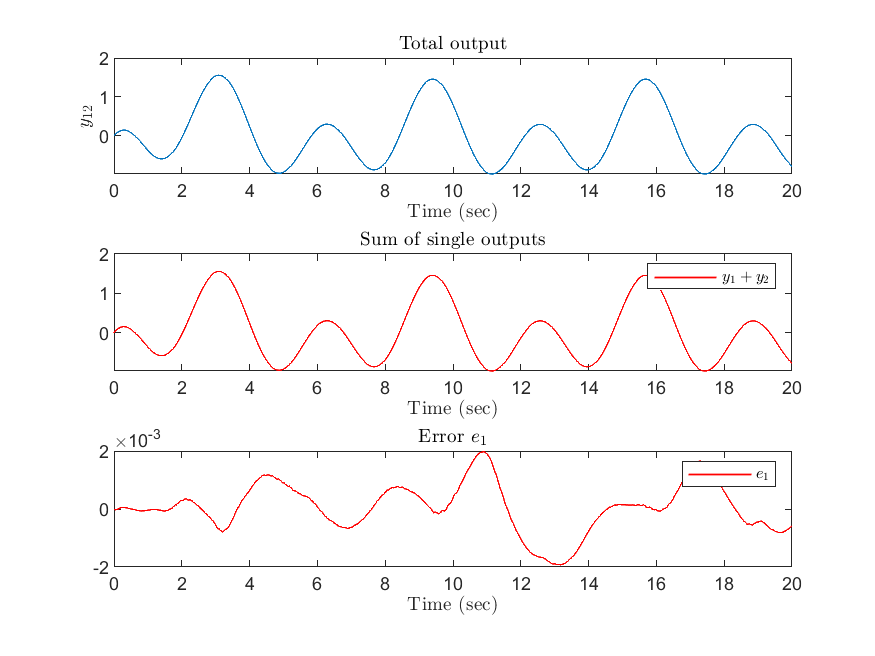
\includegraphics[width=0.6\textwidth]{linear_1st_crit_1.png}
    \caption{\label{fig:lin1_1}Σφάλμα κλίμακας $10^{-3}$ θεωρείται αμελητέο}
    \end{figure}

    \begin{figure}[!htb]
    \centering
    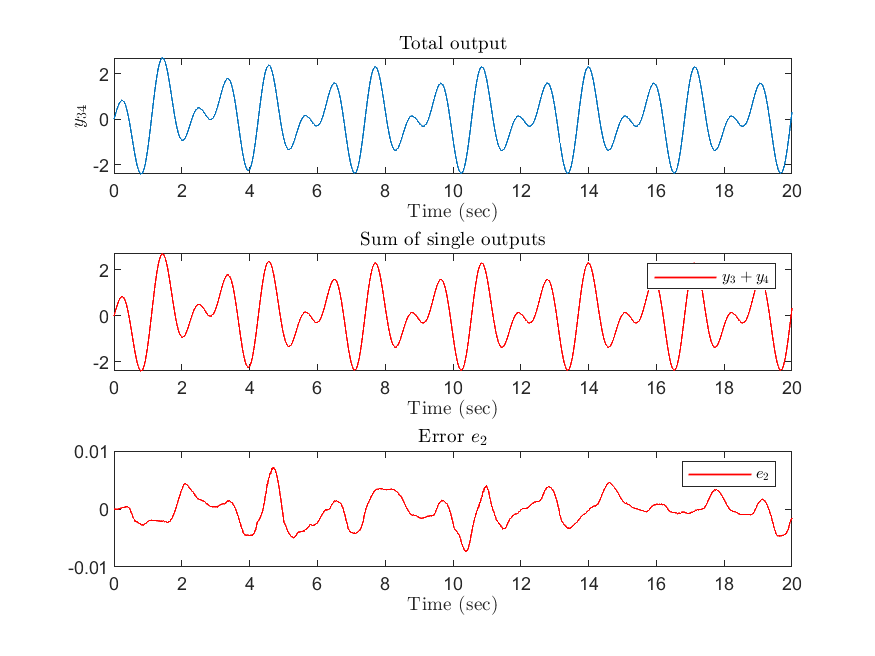
\includegraphics[width=0.6\textwidth]{linear_1st_crit_2.png}
    \caption{\label{fig:lin1_2}Σφάλμα κλίμακας $10^{-2}$ θεωρείται αμελητέο}
    \end{figure}
    
    Ομοίως(σχήμα \ref{fig:lin1_2}) για διαφορετικά μεγέθη και συναρτήσεις εισόδου έχω ανάλογο ικανοποιητικό αποτέλεσμα. Είναι σαφές λοιπόν πως ικανοποιείται το πρώτο κριτήριο γραμμικότητας.    
    
    \item Νόμος H: Έστω οι έξοδοι υπό συντελεστή ομοιογένειας 3
    \begin{equation*}
    y_{tot}(t) = H\left[u_{tot}(t)\right]
    \end{equation*}
    \begin{equation*}
    y_{hom3}(t) = H\left[3 \cdot u_{tot}(t)\right]
    \end{equation*}
    το σύστημα επιβεβαιώνει την αρχή ομοιογένειας αν και μόνο αν: 
    \begin{equation*}
    H\left[3 \cdot u_{tot}(t)\right] = 3 \cdot H\left[u_{tot}(t)\right]
    \end{equation*}

    κατά την προσομοίωση επιλέγουμε τις εισόδους: 
    \begin{equation*}
    \boxed{
    u_{tot} =  0.5 \cdot cos(2 \cdot t) + 3 \cdot sin(5 \cdot t)
    }
    \end{equation*}
    \begin{equation*}
    \boxed{
    u_{hom} = u_1 + u_2 = cos(t) + 2 \cdot cos(2 \cdot t)
    }
    \end{equation*}  

    παίρνουμε τις εξόδους απο το αρχείο \textit{sys.p}:
    \begin{equation*}
    \boxed{
    y_{hom}(t) = T\left[u_{hom}(t)\right]
    }
    \end{equation*}
    \begin{equation*}
    \boxed{
    y_{tot}(t) = T\left[u_{tot}(t)\right]
    }
    \end{equation*}
    ορίζουμε ως σφάλμα την διαφορά εξόδου των σημάτων:
    \begin{equation*}
    e(t) = y_{hom}(t) - 3 * y_{tot}(t)
    \end{equation*}

    για χρόνο:  $ 0 \leq t \leq 20 \enspace$   με βήμα 0.001 sec παρουσιάζεται το σφάλμα τιμών ομοιογένειας συναρτήσει του χρόνου: 
    
    \begin{figure}[!htb]
    \centering
    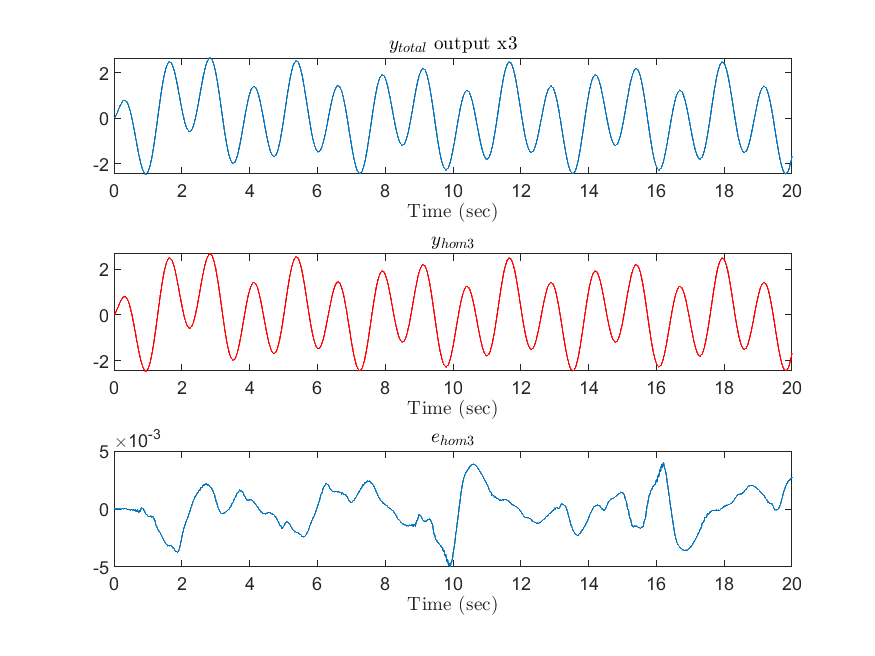
\includegraphics[width=0.6\textwidth]{linear_2nd_crit_1.png}
    \caption{\label{fig:lin2_1}Σφάλμα κλίμακας $10^{-3}$ θεωρείται αμελητέο για συντελεστή ομοιογένειας $=$ 3}
    \end{figure}

    \begin{figure}[!htb]
    \centering
    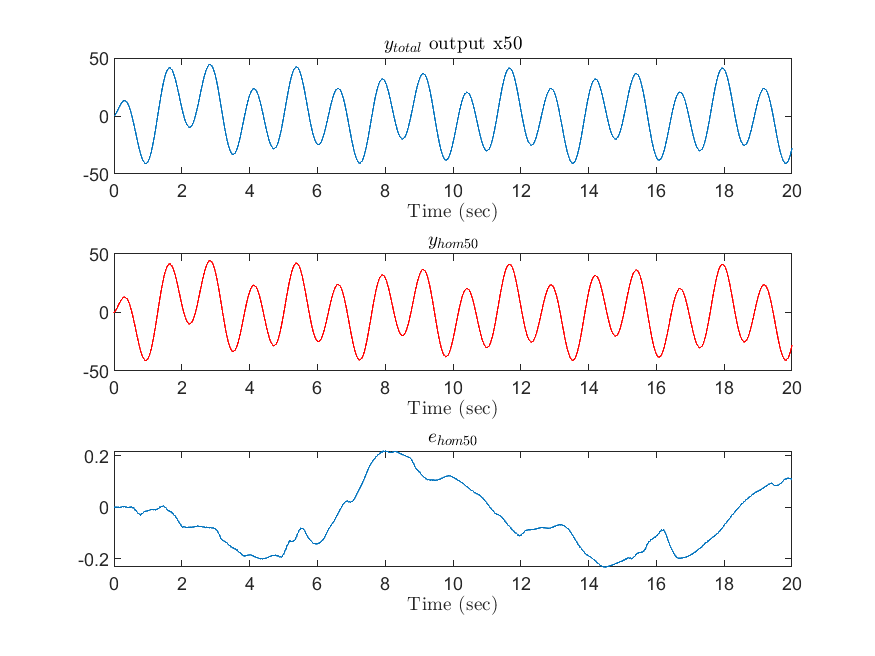
\includegraphics[width=0.6\textwidth]{linear_2nd_crit_2.png}
    \caption{\label{fig:lin2_2}Σφάλμα κλίμακας $10^{-1}$ θεωρείται αμελητέο για συντελεστή ομοιογένειας $=$ 50}
    \end{figure}

    Εύκολα γίνεται αντιληπτή η εξακρίβωση της αρχής της ομοιογένειας των σημάτων στα σχήματα \ref{fig:lin2_1},\ref{fig:lin2_2} και επιβεβαιώνεται το δεύτερο κριτήριο της γραμμικότητας.

\end{itemize}

Προσομοίωση ερωτήματος με MATLAB demo: \textit{testIfLinear.m}.




\section{Ερώτημα Β) Μαθηματική Ανάλυση μεθόδων εκτίμησης παραμέτρων μοντέλου}

Στην προηγούμενη ενότητα αποδείξαμε ότι το σύστημα (S) ακολουθεί γραμμική συμπεριφορά και ξέρουμε ήδη ότι είναι αιτιατό και ευσταθές. Μπορούμε, λοιπόν, να ορίσουμε ότι το μοντέλο συστήματος που θέλουμε να προσεγγίσουμε παραμετρικά και να λύσουμε έχει γραμμική δομή της μορφής: 
\begin{equation*}
% \hspace*{-2.5cm} 
y^{(n)} + θ_0 \cdot y^{(n-1)} + θ_1 \cdot  y^{(n-2)} + ... + θ_{n-1} \cdot  y =  θ_n \cdot u^{(m)} + θ_{n+1} \cdot u^{(m-1)} + θ_{n+2} \cdot u^{(m-2)} + ... +  θ_{n+m} \cdot u 
\end{equation*}
όπου n και m αντίστοιχα οι τάξεις της εισόδου και της εξόδου που επιθυμούμε να βρούμε.

\subsection{i) Μέθοδος μη-πραγματικού χρόνου}

Για την εκτίμηση των παραμέτρων με μια μέθοδο μη-πραγματικού χρόνου, επιλέγουμε τον \textbf{αλγόριθμο των ελαχίστων τετραγώνων}. Επιθυμούμε να φέρουμε το σύστημα στην μορφή
\begin{equation*}
y = {θ_λ}^{\!T}ζ
\end{equation*}
οπου 
\begin{equation*}
{θ_λ} = \begin{bmatrix}
    {{θ_1}^*}^{\!T} - {λ}^{\!T} & {{θ_2}^*}^{\!T}   
     
  \end{bmatrix}^{\!T}
\end{equation*}
\[
{θ_1}^* = \begin{bmatrix}
    θ_0 & θ_1 & θ_2 & ... & θ_{n-1}  
     
  \end{bmatrix}^{\!T}
\]
\[
{θ_2}^* = \begin{bmatrix}
    θ_{n} & θ_{n+1} & θ_{n+2} & ... & θ_{n+m}   
     
  \end{bmatrix}^{\!T}
\]
και για κάθε περίπτωση επιλέγουμε ένα ευσταθές φίλτρο n ταξής της μορφής
\begin{equation*}
Λ(s) = (s + pole)^n = s^n + λ^{Τ} Δ_{n-1}
\end{equation*}
\begin{equation*}
λ = [\enspace λ_1 \enspace λ_2 \enspace ... \enspace λ_n \enspace ] ^{Τ}
\end{equation*}

κατά τα γνωστά συμφωνα με την θεωρία
\begin{equation*}
\zeta = \begin{bmatrix}
-\frac{{Δ^{Τ}}_{n-1}(s)}{Λ(s)}  y & \frac{{Δ^{Τ}}_{m}(s)}{Λ(s)}u  
\end{bmatrix}
\end{equation*}

Συνεπώς, αυτό που απαιτείται στην μοντελοποίηση ενός συστήματος κατά μαύρου κουτιού είναι να υποθέσουμε τις άγνωστες τάξεις εισόδου και εξόδου.
Παρακάτω παρουσιάζεται μια σειρά δοκιμών σε μια λούπα που έγινε για την επιλογή της τάξης εισόδου και εξόδου του συστήματος.
\par Στην \hyperref[sec:validation]{τέταρτη} ενότητα της εργασίας θα γίνει και η αξιολόγηση των διαγραμμάτων και των συντελεστών μέτρησης μας για κάθε προσομοίωση μοντέλου. 
\begin{center}
\begin{tabular}{ |c|c|c| } 
 \hline
$\qquad$ $\qquad$ Δοκιμές $\qquad$ $\qquad$ &$\qquad$ n $\qquad$& $\qquad$ m $\qquad$ \\ 
  \hline
 $1^{η}$ δοκιμή & 2 & 1 \\ 
  \hline
  $2^{η}$ δοκιμή & 3 & 1 \\ 
  \hline
   $3^{η}$ δοκιμή & 3 & 2 \\ 
  \hline
   $4^{η}$ δοκιμή & 4 & 1 \\ 
  \hline
   $5^{η}$ δοκιμή & 4 & 2 \\ 
  \hline
   $6^{η}$ δοκιμή & 4 & 3 \\ 
  \hline
  $7^{η}$ δοκιμή & 5 & 1 \\ 
  \hline
  $8^{η}$ δοκιμή & 5 & 2 \\ 
  \hline
  $9^{η}$ δοκιμή & 5 & 3 \\ 
  \hline
  $10^{η}$ δοκιμή & 5 & 4 \\ 
  \hline
\end{tabular}
\end{center}
\par Τα διαγράμματα που ακολουθούν στο σχήμα \ref{fig:offEst} είναι γραφικές παράστασείς του σφάλματος εκτίμησης εξόδου:
\begin{equation*}
error = y_{real} - y_{estimated} = y - \hat{y}
\end{equation*}
όπου: 
\begin{itemize}
\item $y_{real}$ είναι οι τιμές εξόδου του πραγματικου σύστημος που μας επιστρέφει το αρχείο \textbf{sys.p}
\item $y_{estimated}$ είναι οι τιμές που προέκυψαν απο το γινόμενο του πίνακα παραμέτρων (αποτέλεσμα του αλγόριθμου ελαχίστων τετραγώνων) με τον πίνακα οπισθοδρομητών $\zeta$.   
\end{itemize}
% \large

\begin{figure}[!htb]
    \centering
    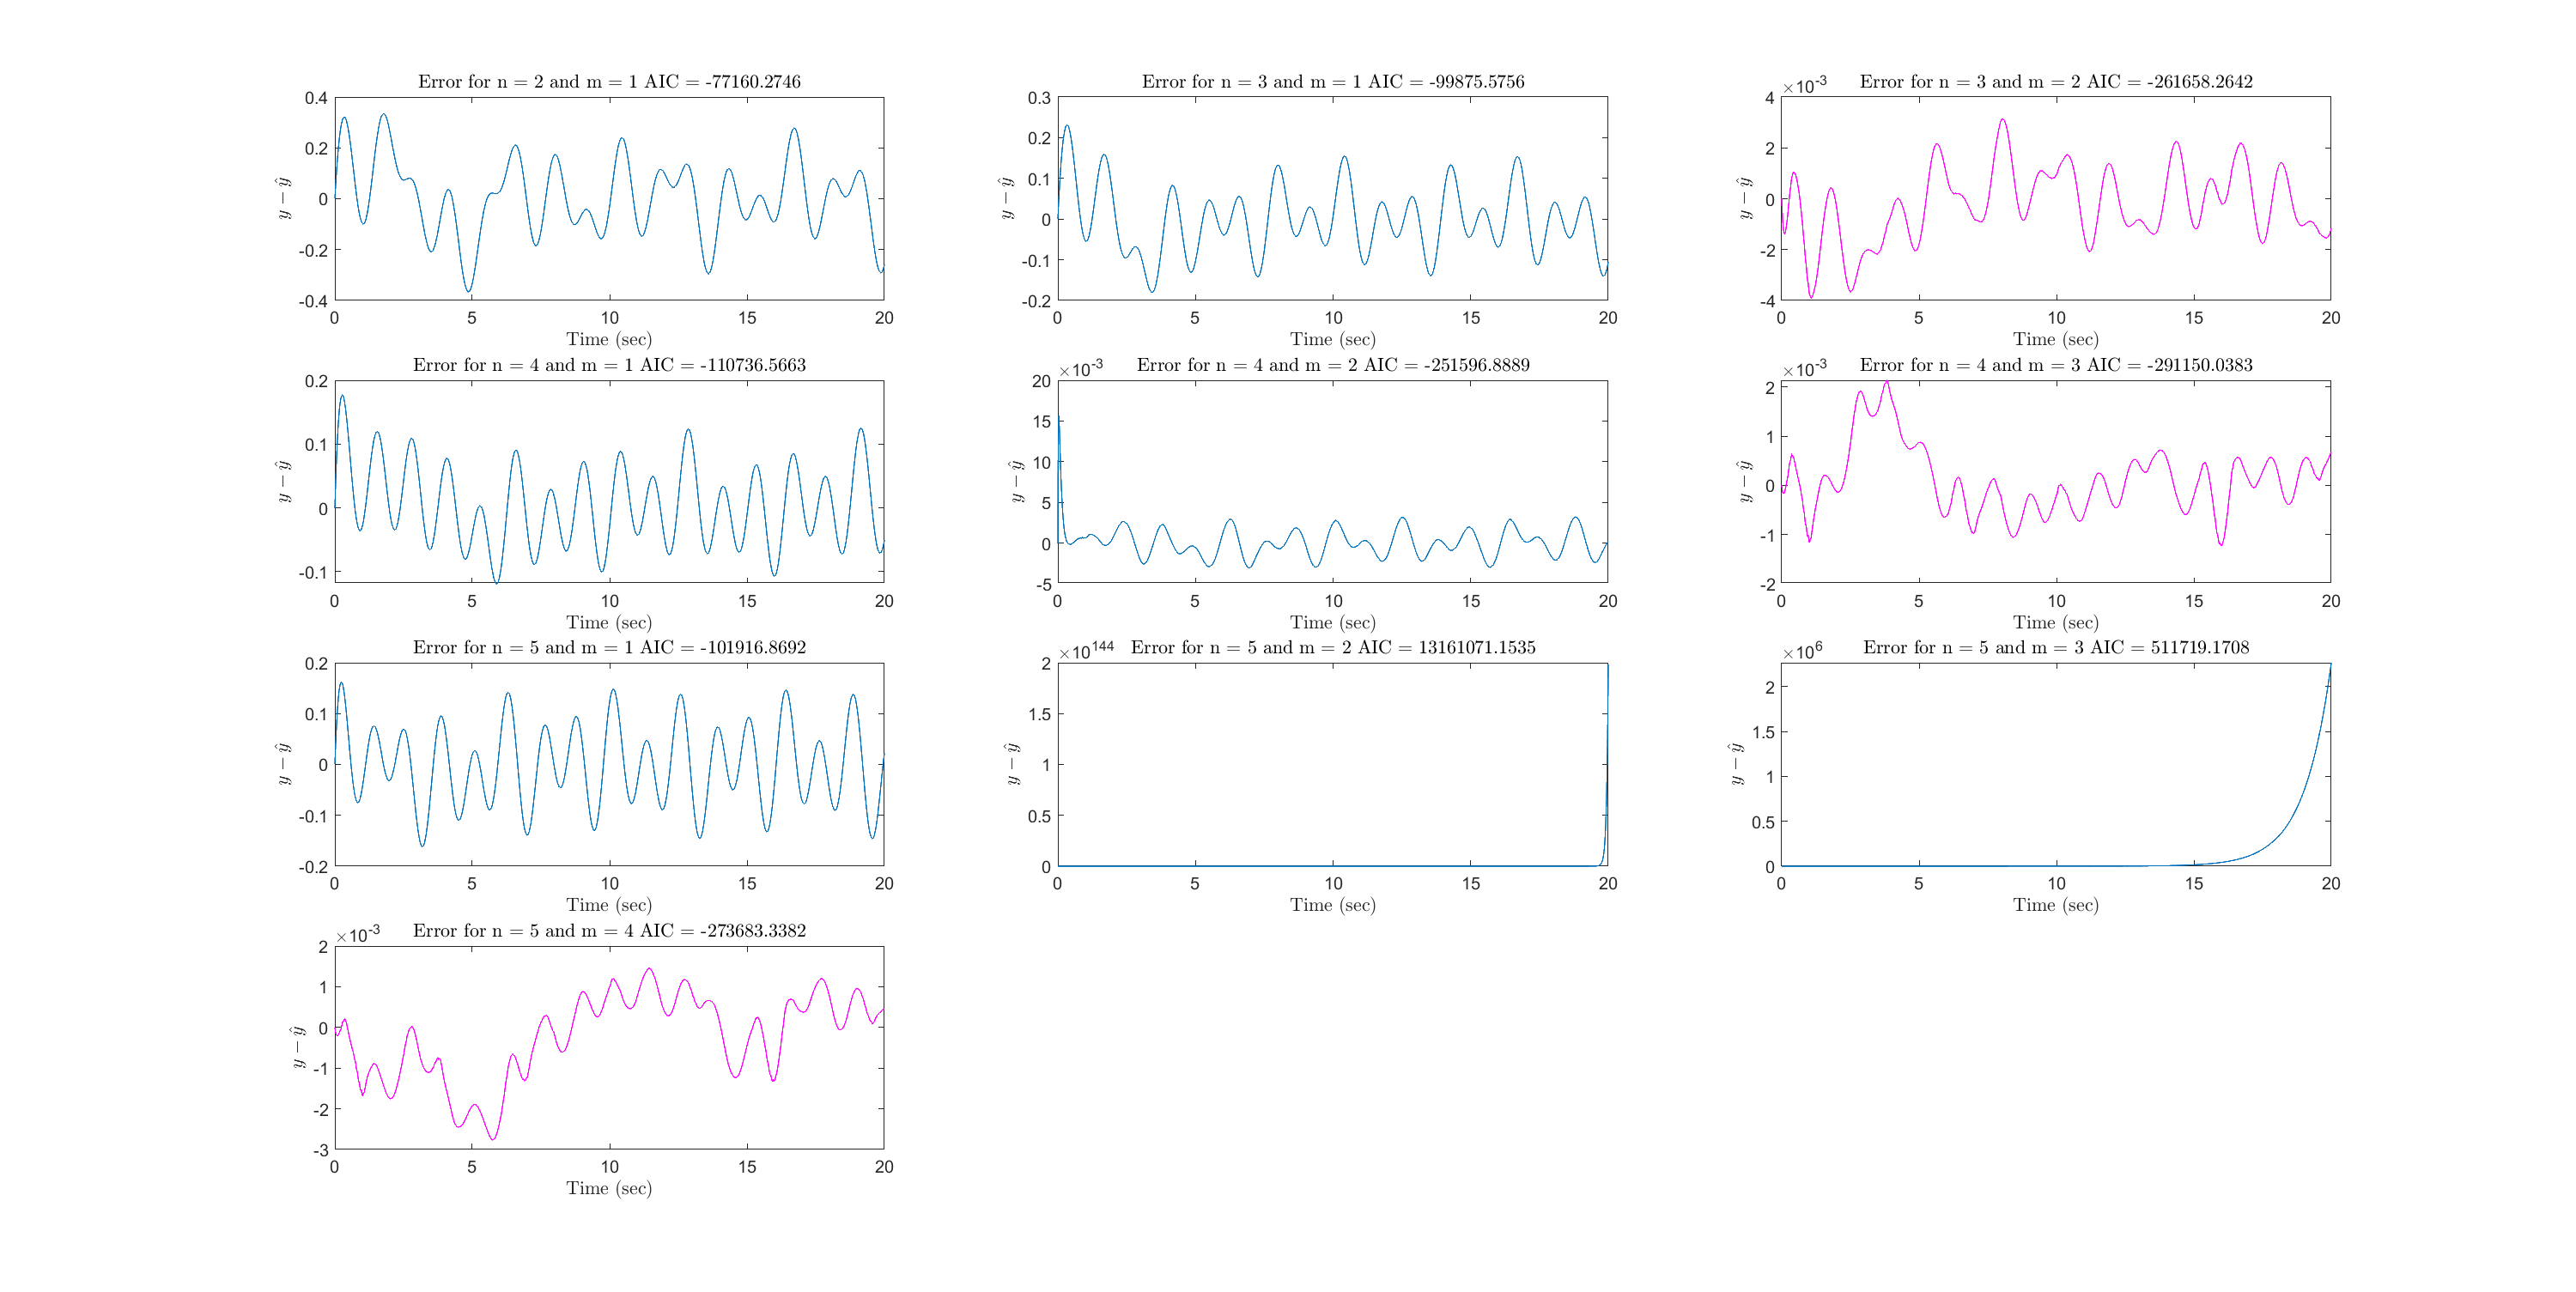
\includegraphics[width=1.1\textwidth]{offlineEstimation.png}
    \caption{\label{fig:offEst}Σφάλματα τιμών με την μέθοδο μη-πραγματικού χρόνου αλγορίθμου ελαχίστων τετραγώνων}
    \end{figure}

Προσομοίωση ερωτήματος με MATLAB demo: \textit{offlineEstimation.m}.

\subsection{ii) Μέθοδος πραγματικού χρόνου}

Για την εκτίμηση των παραμέτρων με μια μέθοδο πραγματικού χρόνου, επιλέγουμε τον \textbf{αναδρομικό αλγόριθμο των ελαχίστων τετραγώνων}. Επιθυμούμε να φέρουμε το σύστημα στην μορφή
\begin{equation*}
y = {θ^*}^Tφ
\end{equation*}
όπου $y$ η έξοδος, ${θ^*}$ το διάνυσμα των άγνωστων αλλά σταθερών παραμέτρων και $\phi$ το διάνυσμα των οπισθιδρομητών. Τόσο η έξοδος όσο και το $\phi$ είναι μετρήσιμα. \par Έστω το σύστημα αναγνώρισης:
\begin{equation*}
\hat{y} = \hat{{θ}^T}φ 
\end{equation*}
όπου $\hat{y}$ η εκτιμώμενη έξοδος και $\hat{θ}$ το διάνυσμα των εκτιμώμενων παραμέτρων.
\par Το σφάλμα αναγνώρισης ορίζεται ως:
\begin{equation*}
\tilde{y} = y - \hat{{θ}^T}φ 
\end{equation*}
\par Θέλουμε να υπολογίσουμε την τιμή $\hat{θ}$ που θα ελαχιστοποιεί το κριτήριο:
\begin{equation*}
K(\hat{θ}) = \frac{1}{2}e^{-βt}(\hat{θ}(t) - \hat{θ}(0))^T Q_0 (\hat{θ}(t) - \hat{θ}(0)) + \frac{1}{2} \int_{0}^{t} e^{-β(t-τ)}[y(τ) - \hat{θ}(t)^Tφ(τ)]^2 dτ
\end{equation*}
όπου $Q_0$ = ${Q_0}^T$ (θετικά ορισμένος πίνακας), β$\geq$0 μια σταθερά. Η Κ($\hat{θ}$) είναι κυρτή συνάρτηση του $\hat{θ}$ . Επομένως κάθε τοπικό ελάχιστο είναι και μοναδκό ολικό και ικανοποιεί:
\begin{equation*}
\nabla{K(\hat{θ})} = 0
\end{equation*}
καταλήγουμε:
\begin{equation*}
\hat{θ}(t) = P(t) [ e^{-βt} Q_0 \hat{θ}(0) + \int_{0}^{t} e^{-β(t-τ)}y(τ)φ(τ) dτ]
\end{equation*}
\begin{equation*}
P(t) = [ e^{-βt} Q_0 + \int_{0}^{t} e^{-β(t-τ)}φ(τ)φ^T(τ) dτ]^{-1}
\end{equation*}
γνωρίζουμε οτι Ρ$P^{-1}$ = Ι οπου Ι ο μοναδιαίος πίνακας συνεπώς:
\begin{equation*}
\frac{d}{dt}[PP^{-1}] = 0
\end{equation*}
λύνοντας ως προς $\dot{P}$:
\begin{equation*}
\dot{P} = -P(\frac{d}{dt}P^{-1})P
\end{equation*}
\begin{equation*}
P^{-1}(t) = e^{-βt} Q_0 + \int_{0}^{t} e^{-β(t-τ)}φ(τ)φ^T(τ) dτ
\end{equation*}
\begin{equation*}
\frac{d}{dt}P^{-1} = -β P^{-1} + φφ^T
\end{equation*}
αντικαθιστώντας βγάζουμε:
\begin{equation*}
\boxed{\dot{P}=βP - Pφ φ^T P}\enspace και\enspace P(0)={Q_0}^{-1}
\end{equation*}
ομοίως:
\begin{equation*}
\hat{θ}(t) = P(t)Ω(t)
\end{equation*}
\begin{equation*}
\dot{Ω} = -βΩ +yφ \enspace Ω(0) = Q_0 \hat{θ}(0)
\end{equation*}
παραγωγίζοντας το $\hat{θ}$ καταλήγουμε:
\begin{equation*}
\boxed{
\dot{\hat{θ}} = P(t)\tilde{y}(t)φ(t)
}
\end{equation*}

\par Αντίστοιχα με την offline μέθοδο πρόκειται να λύσουμε το σύστημα για διάφορες τιμές των n και m. Παρακάτω παρουσιάζεται μια σειρά δοκιμών σε μια λούπα που έγινε για την επιλογή της τάξης εισόδου και εξόδου του συστήματος. 
\begin{center}
\begin{tabular}{ |c|c|c| } 
 \hline
$\qquad$ $\qquad$ Δοκιμές $\qquad$ $\qquad$ &$\qquad$ n $\qquad$& $\qquad$ m $\qquad$ \\ 
  \hline
 $1^{η}$ δοκιμή & 2 & 1 \\ 
  \hline
  $2^{η}$ δοκιμή & 3 & 1 \\ 
  \hline
   $3^{η}$ δοκιμή & 3 & 2 \\ 
  \hline
   $4^{η}$ δοκιμή & 4 & 1 \\ 
  \hline
   $5^{η}$ δοκιμή & 4 & 2 \\ 
  \hline
   $6^{η}$ δοκιμή & 4 & 3 \\ 
  \hline
  $7^{η}$ δοκιμή & 5 & 1 \\ 
  \hline
  $8^{η}$ δοκιμή & 5 & 2 \\ 
  \hline
  $9^{η}$ δοκιμή & 5 & 3 \\ 
  \hline
  $10^{η}$ δοκιμή & 5 & 4 \\ 
  \hline
\end{tabular}
\end{center}

\par Αντίστοιχα με την offline μέθοδο εκτίμησης τα διαγράμματα που ακολουθούν στο σχήμα \ref{fig:onlEst} είναι γραφικές παράστασείς του σφάλματος εκτίμησης εξόδου και στην \hyperref[sec:validation]{τέταρτη} ενότητα της εργασίας θα γίνει και η αξιολόγηση των διαγραμμάτων και των συντελεστών μέτρησης μας για κάθε προσομοίωση μοντέλου:
\begin{figure}[!htb]
    \centering
    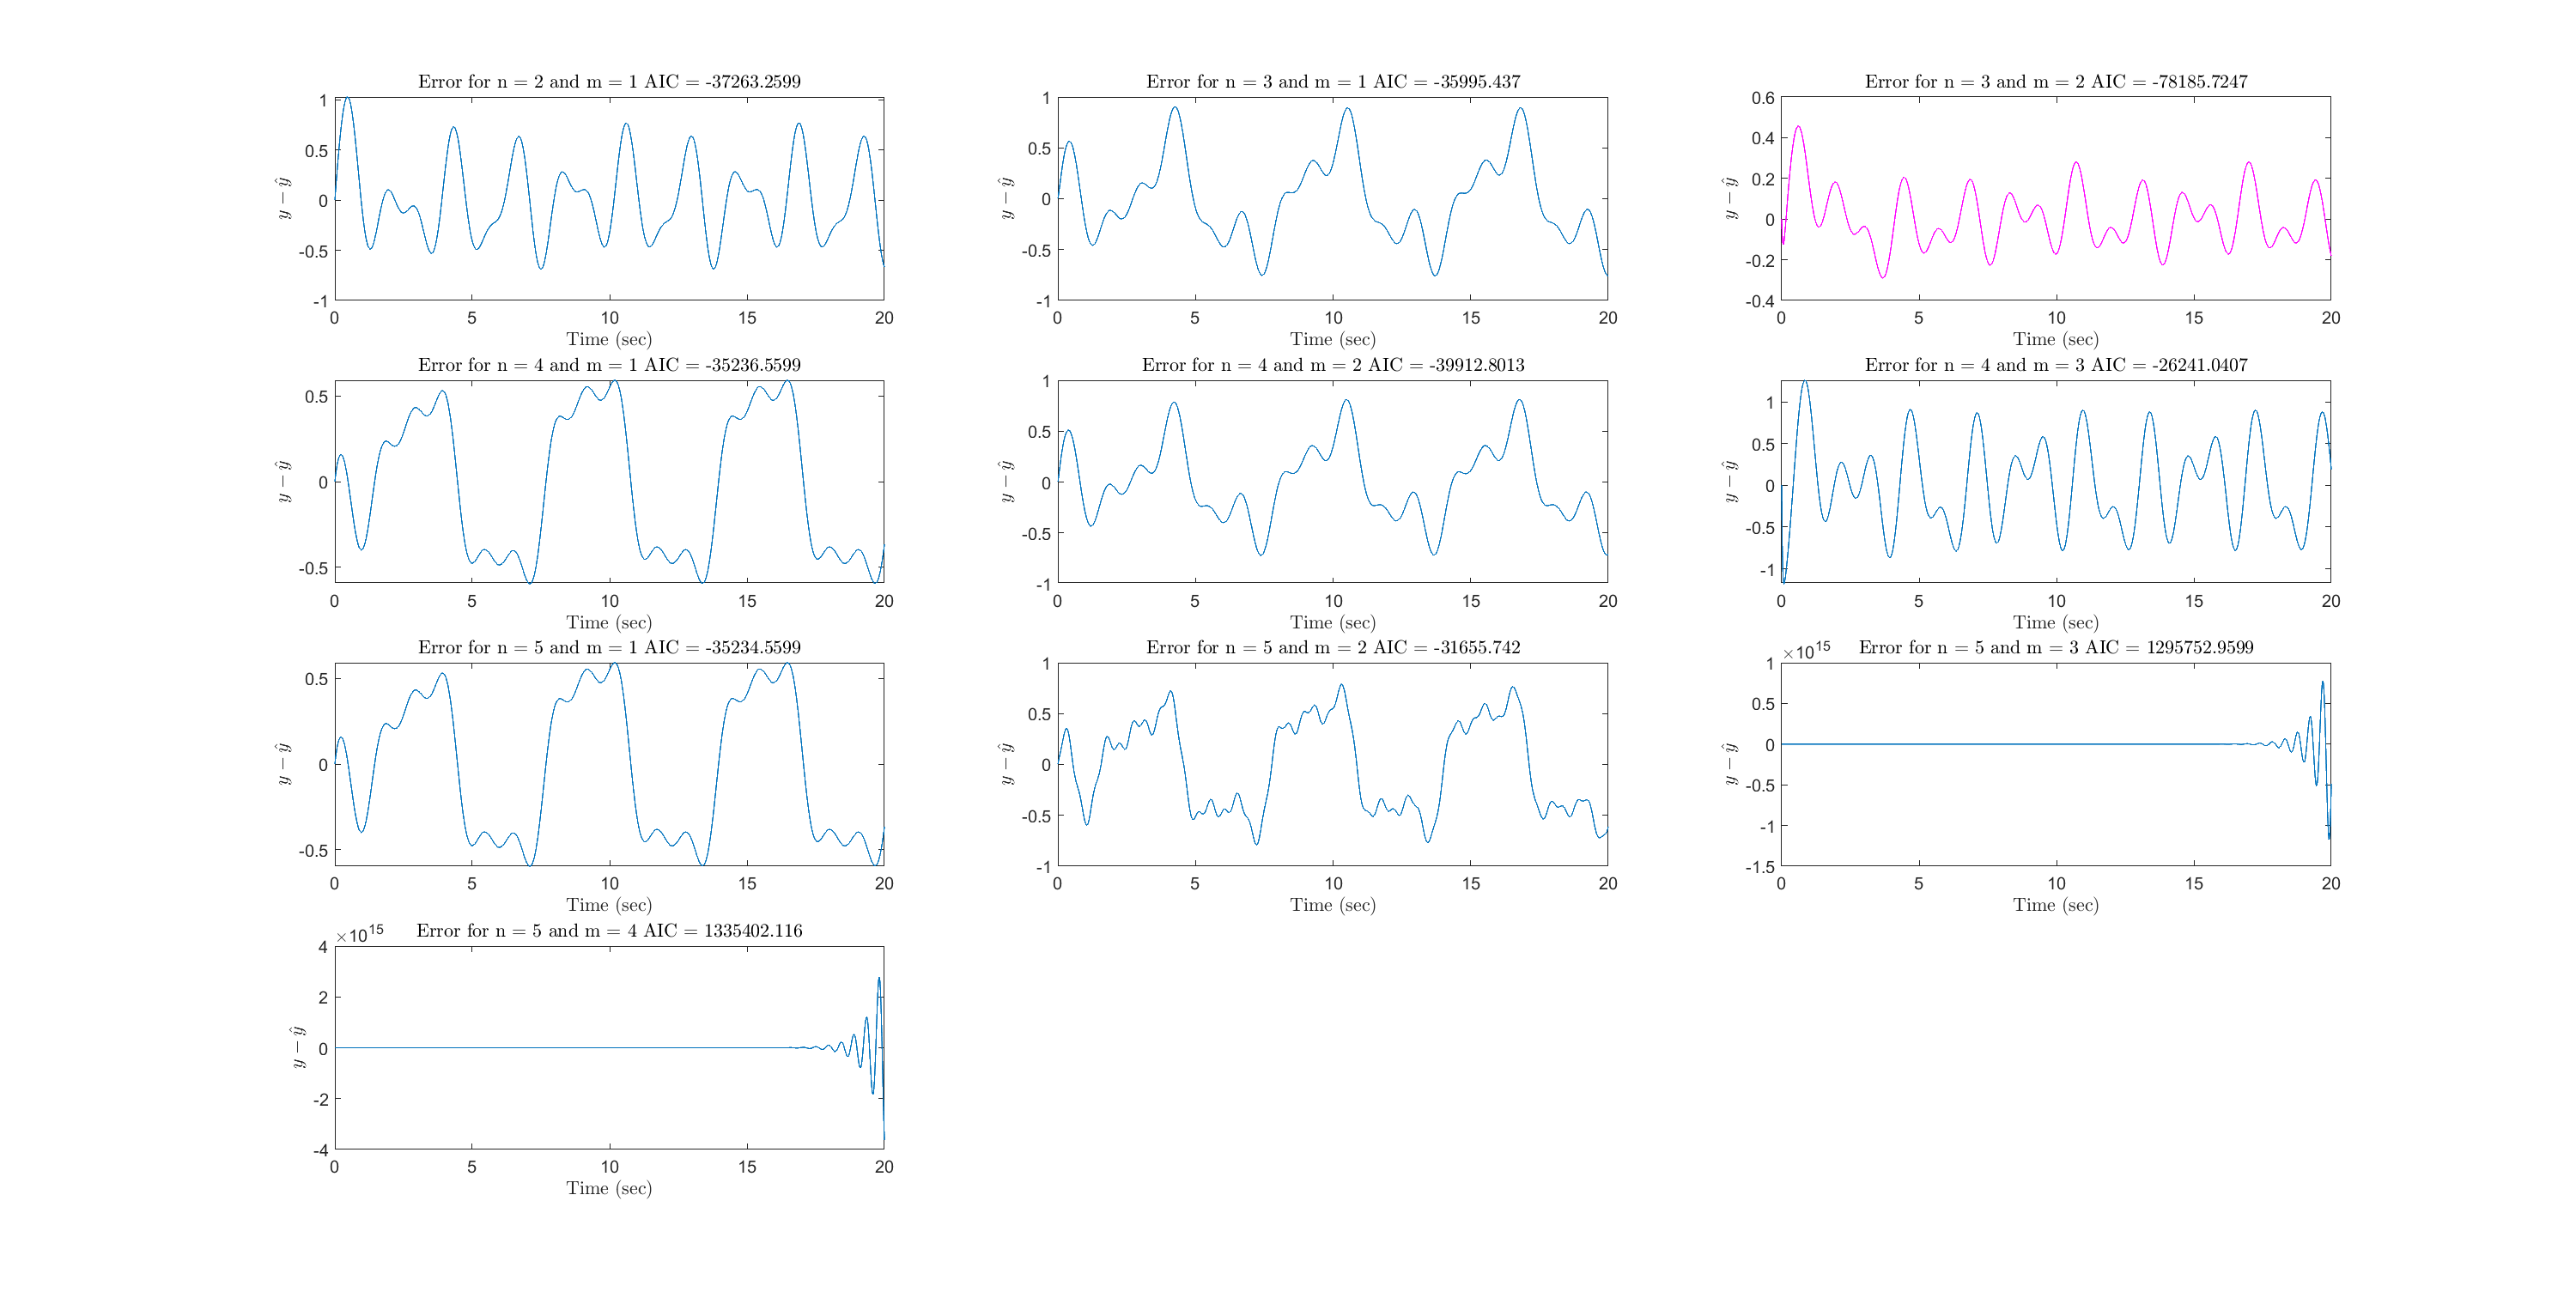
\includegraphics[width=1.1\textwidth]{onlineEstimation.png}
    \caption{\label{fig:onlEst}Σφάλματα τιμών με την μέθοδο πραγματικού χρόνου αναδρομικού αλγορίθμου ελαχίστων τετραγώνων}
    \end{figure}

Προσομοίωση ερωτήματος με MATLAB demo: \textit{onlineEstimation.m}.

\section{Ερώτημα Γ) Αξιολόγηση μοντέλων που αποκτήθηκαν κατά τη διαδικασία αναγνώρισης}
\label{sec:validation}
Κριτήρια αξιολόγησης: 
\begin{itemize}
    \item Σφάλματα των τιμών εξόδου: $e(t) = y_{test} - \hat{y}_{test}$
    \item Κριτήριο πληροφορίας του Akaine($AIC = Nln (I(θ)) + \rho\kappa$), όπου $Ν$ το πλήθος των δεδομένων ελέγχου της δειγματοληψίας, $\kappa = n+m+1$ ο αριθμός των παραμέτρων του συστήματος, $\rho$ μια θετική σταθερά(τυπικά $\rho$=2) και
\begin{equation*}
I(θ)=\frac{1}{N} \sum_{i=1}^{N} \left(y_i-\hat{y}_i \right)^{2}
\end{equation*}
\end{itemize}
Συμπερασματικά βασιζόμενοι στα σχήματα \ref{fig:offEst} και \ref{fig:onlEst} και στα παραπάνω δύο κριτήρια αξιολόγησης που αναγράφονται στο κάθε διάγραμμα των δύο σχημάτων προκύπτει το συμπέρασμα ότι οι μικρότερες τιμές των συντελεστών αξιολόγησής μας προκύπτουν για τον \textbf{συνδυασμό $n = 3$ και $m = 2$}. Αυτό, διότι, επιθυμούμε το μοντελοποιημένο σύστημά μας να μην έχει κάνει overfit τις παραμέτρους του βασιζόμενο σε ένα συγκεκριμένο σήμα εκμάθησης εισόδου $u(t)$, αλλά να ανταποκρίνεται ικανοποιητικά και σε σήματα εισόδου δοκιμών $u_{test}(t)$. Παράλληλα, θέλουμε η πολυπλοκότητα του συστήματος, δηλαδή οι τάξεις εξόδου και εισόδου της γραμμικής δομής να παραμένουν υπολογιστικά χαμηλές(μικρά $n$ και $m$).

\end{document}